\documentclass[tikz,border=8pt]{standalone}

\usepackage[T1]{fontenc}
\usepackage{helvet}
\renewcommand{\familydefault}{\sfdefault}
\usetikzlibrary{arrows.meta,positioning}

\definecolor{ink}{HTML}{232323}
\definecolor{accent}{HTML}{6F2C91}
\definecolor{panel}{HTML}{E6E6E8}
\definecolor{guardfill}{HTML}{F1ECF6}

\begin{document}
\hyphenpenalty=10000
\exhyphenpenalty=10000
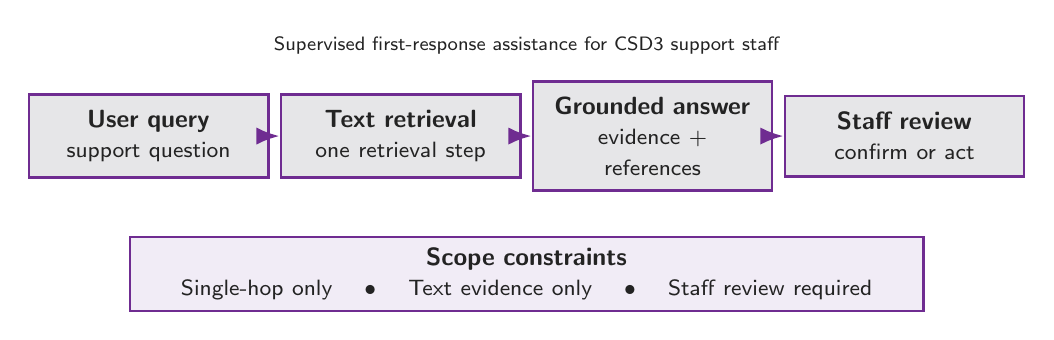
\begin{tikzpicture}[
  font=\small,
  text=ink,
  box/.style={
    draw=accent,
    line width=1.0pt,
    align=center,
    inner sep=5.5pt,
    minimum height=1.02cm,
    text width=2.65cm,
    fill=panel
  },
  support/.style={
    draw=accent,
    line width=0.8pt,
    align=center,
    inner sep=4pt,
    minimum height=0.72cm,
    text width=9.80cm,
    fill=guardfill
  },
  input/.style={box},
  process/.style={box},
  rank/.style={box},
  output/.style={box},
  guard/.style={support},
  arrow/.style={-Latex, very thick, draw=accent},
  meta/.style={font=\scriptsize, text=ink}
]

\node[input] (query) at (0,0) {\textbf{User query}\\{\footnotesize support question}};
\node[process] (retrieve) at (3.20,0) {\textbf{Text retrieval}\\{\footnotesize one retrieval step}};
\node[rank] (answer) at (6.40,0) {\textbf{Grounded answer}\\{\footnotesize evidence + references}};
\node[output] (review) at (9.60,0) {\textbf{Staff review}\\{\footnotesize confirm or act}};

\draw[arrow] (query) -- (retrieve);
\draw[arrow] (retrieve) -- (answer);
\draw[arrow] (answer) -- (review);

\node[guard] (constraints) at (4.80,-1.75) {\textbf{Scope constraints}\\{\footnotesize Single-hop only \quad $\bullet$ \quad Text evidence only \quad $\bullet$ \quad Staff review required}};

\node[meta] at (4.80,1.15) {Supervised first-response assistance for CSD3 support staff};

\end{tikzpicture}
\end{document}
